% This is a default-selection of plugins that are used widely in this repo.

\documentclass[a4paper,10pt,fleqn]{article}
\usepackage[utf8]{inputenc}

% deutsche Trennmuster etc.
\usepackage[ngerman]{babel}
\usepackage[T1]{fontenc}

% mathematical simbols and fonts
\usepackage{mathtools} 
\usepackage{amssymb}
\usepackage{amsmath}
\usepackage{ntheorem}
\usepackage{polynom}
\usepackage{marvosym}
\usepackage{tabu}
\renewcommand*{\bmod}{\mathbin{\%}}
\everymath{\displaystyle}

\usepackage{multicol}
\usepackage{color}
\usepackage[usenames,dvipsnames]{xcolor}
\setlength{\columnsep}{1cm}
\setlength{\columnseprule}{0.25pt}
\def\columnseprulecolor{\color{gray}}
\usepackage{hyperref}

\usepackage[margin=1.5cm]{geometry}
\usepackage{graphicx}
\usepackage{pgfplots}
\pgfplotsset{compat=1.10}

%Code higlighting

\usepackage{minted}

% make lists more compact:
\newlength{\wideitemsep}
\setlength{\wideitemsep}{.5\itemsep}
\addtolength{\wideitemsep}{-5pt}
\let\olditem\item
\renewcommand{\item}{\setlength{\itemsep}{\wideitemsep}\olditem}
\renewcommand{\arraystretch}{1.25}

\title{Zusammenfassung InfSi1}
\author{Fabian Hauser}
 
\begin{document}
\maketitle

\section{Grundbegriff Sicherheit}

Sicherheit: Confidentiality, Integrity, Availability ("CIA")

\begin{description}
\item[Datensicherheit] \hfill \\
	Schutz vor Missbrauch der Daten durch organisatorische und technische Massnahmen
\item[Datenschutz] \hfill \\
	Schutz vor dem Missbrauch ihrer personenbezogenen Daten
\end{description}

\subsection{Management}
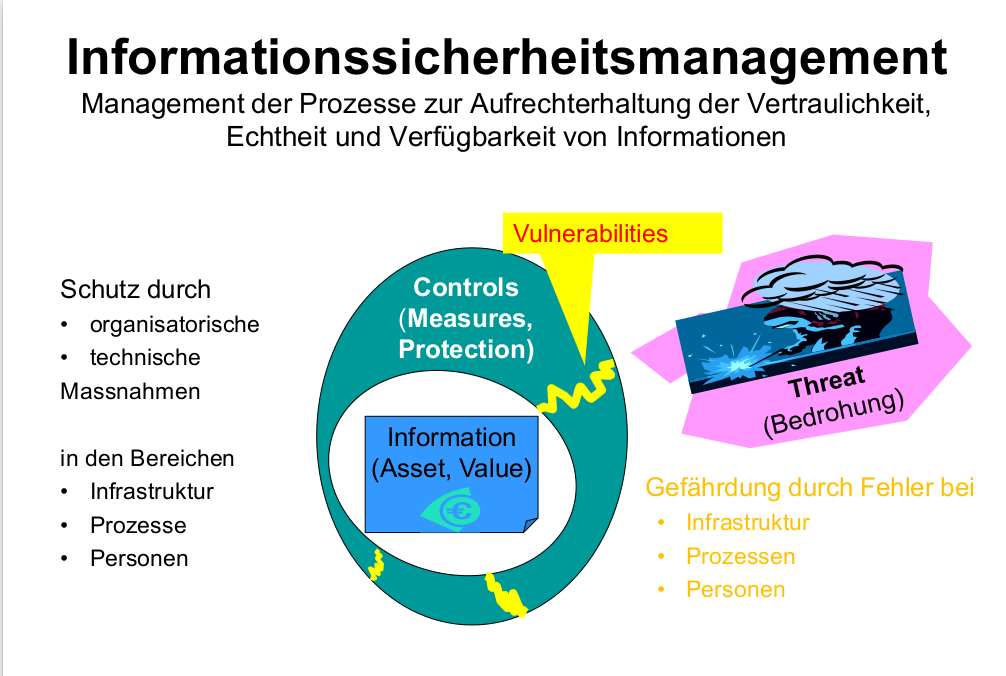
\includegraphics[scale=0.25]{img/informationssicherheitsmanagement.png}

\begin{description}
\item[Threads] \hfill \\
	Wahrscheinlichkeit eines Zwischenfalls * Schaden = Bedrohung * Verletzlichkeit * Schaden
\item[Vulnerabilities]
\item[Control] \hfill \\
	(measures, protection)
\item[Information] \hfill \\
	(asset, value)
\item[Gefährdung] \hfill \\
	(Hazard, Applied thread): Bedrohung + Schwachstelle
\end{description}


\subsection{Massnahmenkataloge}
\begin{enumerate}
\item	Infrastruktur
\item	Organisation
\item	Personal
\item	Hardware/Software
\item	Kommunikation
\item	Notfallvorsorge
\end{enumerate}

\subsection{Gefährdungskataloge (Applied Threat)}
\begin{enumerate}
\item	Höhere Gewalt
\item	Organisatorische Mängel
\item	Mengschliche Fehlhandlungen
\item	Technisches Versagen
\item	Vorsätzliche Handlungen
\end{enumerate}

\subsection{Risikomanagement}

NVD/CVE nach CVSS:	http://www.security-database.com/cvss.php


\section{Standards}

\begin{description}
\item[Formale Standards] \hfill \\
	offizielle Standards, z.B. von Internationalen Standards (ISO, IEC, ITU), Berufsverbänden(IEEE), Staatsstellen NIST
\item[Public (open) Standards] \hfill \\
	Open Source Standards (Internet RFCs)
\item[De-Facto Standards] \hfill \\
	Herzstellerspezifische Standards (z.B. MS Office, PDF, Industriestandards (DIX, ECMA)
\item[Interne Standards] \hfill \\
	(firmeninterne Standards)
\end{description}
	
\subsection{Verbindlichkeiten in Standards}
gemäss RFC 2119:

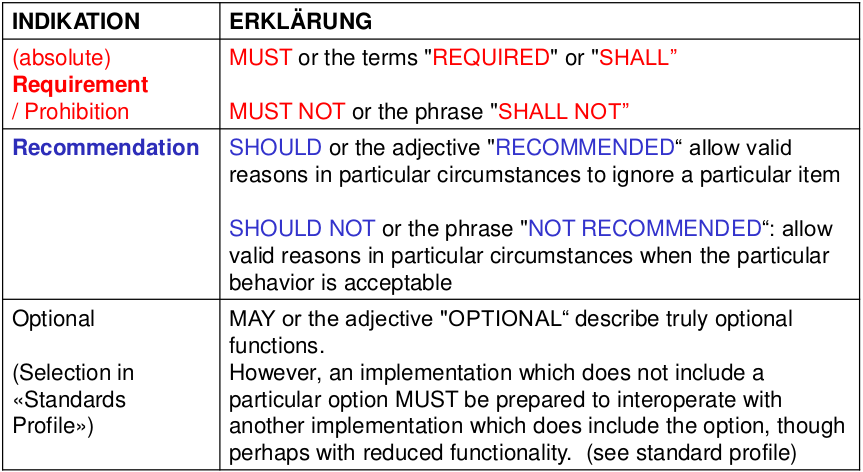
\includegraphics[scale=0.5]{img/rfc2119.png}
	
\subsection{ISO 27000}

\subsubsection{ISO 27001}
	Gibt an, was zu tun ist.
\subsubsection{ISO 27002}
	Enthält Umsetzungshinweise.

\subsection{ITIL}
	Stark angelehnt an \emph{ISO 27001}, um Sicherheit im IT Bereich zu erreichen.


\subsection{OWASP}	
	Open Web Application Security Project.
	
	Bietet Guidlines zur Verbesserung der Sicherheit von Web Applications.

\subsection{Gefährdungen}
\begin{description}
\item[Zero day exploit / attack] \hfill \\
	vulnerability that is unknown to the software vendor
\item[Spear phishing] \hfill \\
	targeted phishing to steal intellectual property, financial data, trade or military secrets and other confidential data.
\item[Advanced persistent threat (APT)] \hfill \\
	stealthy and continuous computer hacking processes, orchestrated by human(s), targeting a specific entity (organizations and/or nations) for business or political motives.
\end{description}

\subsection{Security ...}

 \begin{itemize}
 	\item Übersicht schaffen, Ziele festlegen, Checkliste/Standards nutzen
 	\item Trennung/Separierung von Systemen und Funktionen
 	\item Arbeitsanweisungen, Richtlinien, Regelungen erstellen
 	\item Ausbildung und Sensibilisierung Mitarbeiter
 	\item Kontrollen/Konsequenzen von Verstössen festlegen
 \end{itemize}

\paragraph{Objekte}
	\begin{itemize}
		\item Eigene Informationen
		\item Fremde Informationen
		\item Personen
		\item Gebäude, Räume
		\item Netze
		\item Server
	\end{itemize}

\paragraph{Grundsätzliche Prinzipien der Zugangskontrollen}

\begin{itemize}
	\item Principle of least priviledge / Need to know
	\item Same Origin Policy
	\item Sandbox
	\item Erlaubnis mit Verbotsvorbehalt (Blacklist, opt out)
	\item Verbot mit Erlaubnisvorbehalt (Whitelist, opt in)
	\item Vier-Augen-Prinzip
\end{itemize}


\section{Kryptografie}

%TODO: Formeln Wahrscheinlichkeit


\subsection{Symmetric Encryption}

\subsubsection{Stream Cipher Principle}
Via PRNG wird Cipher Stream generiert und via XOR mit dem Plaintext verknüpft.

\subsubsection{Block Cipher}
Key und Plaintext wird mit einer Encipher-Funktion verarbeitet. Dies wird jeweils auf Blöcke angewendet.

\paragraph{Counter Mode}
Eine Block Cipher generiert für den gleichen Input immer den gleichen Output.
z.T. wird auch ein Counter als Input genommen.

\paragraph{Feedback Mode (CFB)}

Aus dem Initialization Vector und dem Key wird ein BCE-Code generiert, und mit dem XOR kombiniert; dies wird danach wiederum als XOR eingesetzt.


Block Ciphers können auch als generatoren für Bit-Streams verwendet werden, dann ist die Rede von:
\begin{itemize}
	\item Counter Mode
	\item Feedback Mode
\end{itemize}

\subsubsection{PRNG}
Linear Feedback Shift Register (LFSR)
Oft werden mehrere Schieberegister kombiniert, theoretisch wiederholt sich so ein Code nach dem KGV von je $2^n-1$ der Grösse.

\subsection{Informationsgehalt}

\[
	I(x) = \mathrm{ld} \left(Zeichenanzahl \right)
\]

\subsection{RSA Algorithm}

\begin{enumerate}
\item Zwei Primzahlen wählen und Produkt bilden: $n = p \cdot q$
\item $\phi(n) = (p - 1) \cdot (q - 1)$
\item Beliebige Zahl $a$ zwischen 0 und $ \phi(n)$ wählen. Zahl a muss teilerfremd zu $\phi(n)$ sein. $(ggt(\phi(n), a) = 1)$ am besten eignen sich Primzahlen für a. (privater Schlüssel)
\item Multiplikative Inverse b berechnen (öffentlicher Schlüssel)$(a \cdot b = 1 \mod \phi (n))$ Euklidischer Algorithmus
a) Öffentlicher Schlüssel: $n$ und $b$
b) Privater Schlüssel: $a$
\end{enumerate}

\paragraph{Verschlüsseln}
\begin{enumerate}
	\item $\text{Wert}_\text{verschlüsselt} = (\text{Wert}_\text{unverschlüsselt}) b \cdot \mod (n)$
\end{enumerate}

\paragraph{Entschlüsseln}
\begin{enumerate}
	\item $\text{Wert}_\text{unverschlüsselt} = (\text{Wert}_\text{verschlüsselt}) a \cdot \mod(n)$
\end{enumerate}

\subsection{Hashes}

Werden zur Integritätsprüfung (Modification Detection Code, MDC) und Authentizitätsprüfung (Message Authentication Code (MAC) und Digitale Signatur)

Da der Hash üblicherweise kleiner Als die gehashte Nachricht ist, muss es zwangsläufig Doppelbelegungen geben.

Hashes sind Einwegfunktionen.

\subsubsection{Anforderung an crypto-hashfunctions}

One Way (easy, other way hard)
Collision-resistant (hard to find two arbitrary hashes)
Preimage resistant 

\subsubsection{SHA / MD Verfahren}

%TODO: Insert screenshots of presentation 18.04.2016 / page ~20


MD4- und MD5 gelten als gebrochen. SHA-1 nicht mehr empfohlen.

Requirement:
\begin{itemize}
	\item Fast, but not too fast
	\item Avalanche effect (Small change in input, bit change in hash)
	\item Collisions (two files with same hash may not be forged artificially)
\end{itemize}

Möglichkeit, um Brute-Force zu erschwehren: Hash mehrere male anwenden.

\subsection{PKI}

Eine Drittperson verifiziert die Echtheit eines Schlüssels.

\subsubsection{TLS Extensions}

\paragraph{Root CA}
\begin{itemize}
	\item	Root CA
	\item	certificateSign
	\item	crlSign
\end{itemize}

\paragraph{Intermediate CA}
\begin{itemize}
	\item	Intermediate CA
	\item	certificateSign
	\item	crlSign
\end{itemize}

\paragraph{End Certificate}
\begin{itemize}
	\item	End Entity Certificates
	\item	digitalSignature
	\item	nonRepudiation
	\item	keyEncipherment
	\item	dataEncipherment
	\item	keyAgreement
\end{itemize}

\subsubsection{Web of Trust}

Freunde unterschreiben sich Schlüssel gegenseitig.


\subsection{TLS}

\subsubsection{Diffie-Hellman}


\section{AAA}

Authentication, Authorization, Accounting

Bei Windows üblicherweise AD.

\subsection{Authentication}
Username, Password etc.

\subsubsection{Authentication is based on what you...}
\begin{description}
	\item[know]	Password, PIN, secret
	\item[have]	Certificate, Token, Scratch list
	\item[are]	Biological pattern.
\end{description}

Nonce: Einmalig verwendeter Wert (kann auch Counter sein,oder genügend lange random number.)

\subsection{Authorization}
User Rights


\subsection{Accounting}
Logging etc.


\section{File and Disk Encryption}

\subsection{Mittels CBC}
Damit von einem beliebigen Vektor entschlüsselt werden kann, wird aus der Sektornummer der Schlüssel generiert. Problem: Wiederholende Schlüssel für die gleichen Daten.


Watermarking: Datei unterjubeln, welche im Nachhinein nachweisen kann.


Encrypted Salt Sector IV (ESSIV): Verhindert Watermarking durch Verknüpfen Sektornummer mit einem IV.


Problem: Diverse angriffe, wenn nicht alles gechained verknüpft wird, was aus performancegründen nicht geht.

\subsection{XTS}

Jeder AES-Block hat eine individuelle Maske 

\section{E-Mail Encryption}

Signature and Encryption

PKCS\#7


\section{Prüfungsinfos}

Modulprüfung: Mo, 15.8.2016
10:30-12:30, HSR 4.101 (Aula)

\begin{itemize}
\item Ohne Unterlagen \& Rechner (Formeln werden z.T. abgegeben)
\item Aufgaben an Notebook:
\item Webanwendung, Wireshark, Cryptool
\item Lernkontrolle-Account muss bereit sein
\item Persönliches Zertifikat zur S/MIME für Mail Signatur/Verschlüsselung
\end{itemize}

- Test: Hinter den Kulissen der WhatsApp-Verschlüsselung (Heise online security.)

BSI TR-02102

\url{https://www.bsi.bund.de/DE/Publikationen/TechnischeRichtlinien/tr02102/index_htm.html}

http://tlng.cnlab.ch/mobilequiz_v3/
\end{document}